Hallar el volumen del sólido que se genera al girar la región comprendida entre las curvas $y=8x^2$ y $y=\sqrt{8x}$ alrededor del eje $x$.

\nopagebreak
\begin{align*}
\text{Intersección: } 8x^2 = \sqrt{8x} \implies 64x^4 = 8x \implies 8x(8x^3-1)=0. \\
x=0, x=1/2. \\
\text{En } [0, 1/2], \sqrt{8x} \ge 8x^2. \\
V &= \pi \int_{0}^{1/2} ((\sqrt{8x})^2 - (8x^2)^2) \, dx \\
&= \pi \int_{0}^{1/2} (8x - 64x^4) \, dx \\
&= \pi \left[ 4x^2 - \frac{64x^5}{5} \right]_{0}^{1/2} \\
&= \pi \left( 4(1/4) - \frac{64(1/32)}{5} \right) = \pi (1 - 2/5) = \frac{3\pi}{5}
\end{align*}

\[
\boxed{\displaystyle \frac{3\pi}{5}}
\]

\begin{center}
    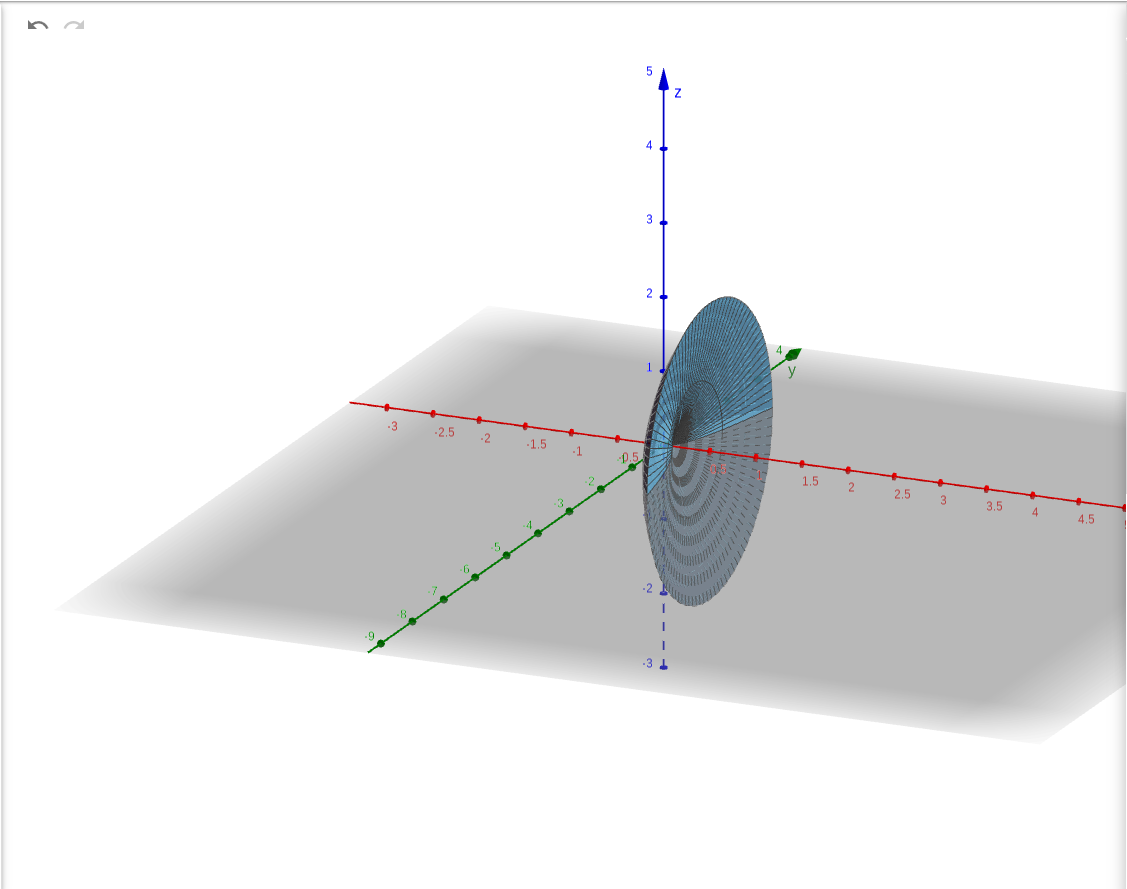
\includegraphics[width=0.5\textwidth]{Graficas/ejer36.png}
\end{center}
